\section{Taxonomy of Multimodal Time Series Models}
\label{sec:taxonomy}

To provide a rigorous structural foundation for this survey, we propose a multi-dimensional taxonomy deconstructing the literature across four orthogonal pillars: (1)~\textbf{Modality Pairing}, (2)~\textbf{Fusion Architecture}, (3)~\textbf{Functional Role of the Complementary Modality}, and (4)~\textbf{Downstream Tasks and Domains} (illustrated in \Cref{fig:taxonomy}).

\begin{figure*}[t]
\centering
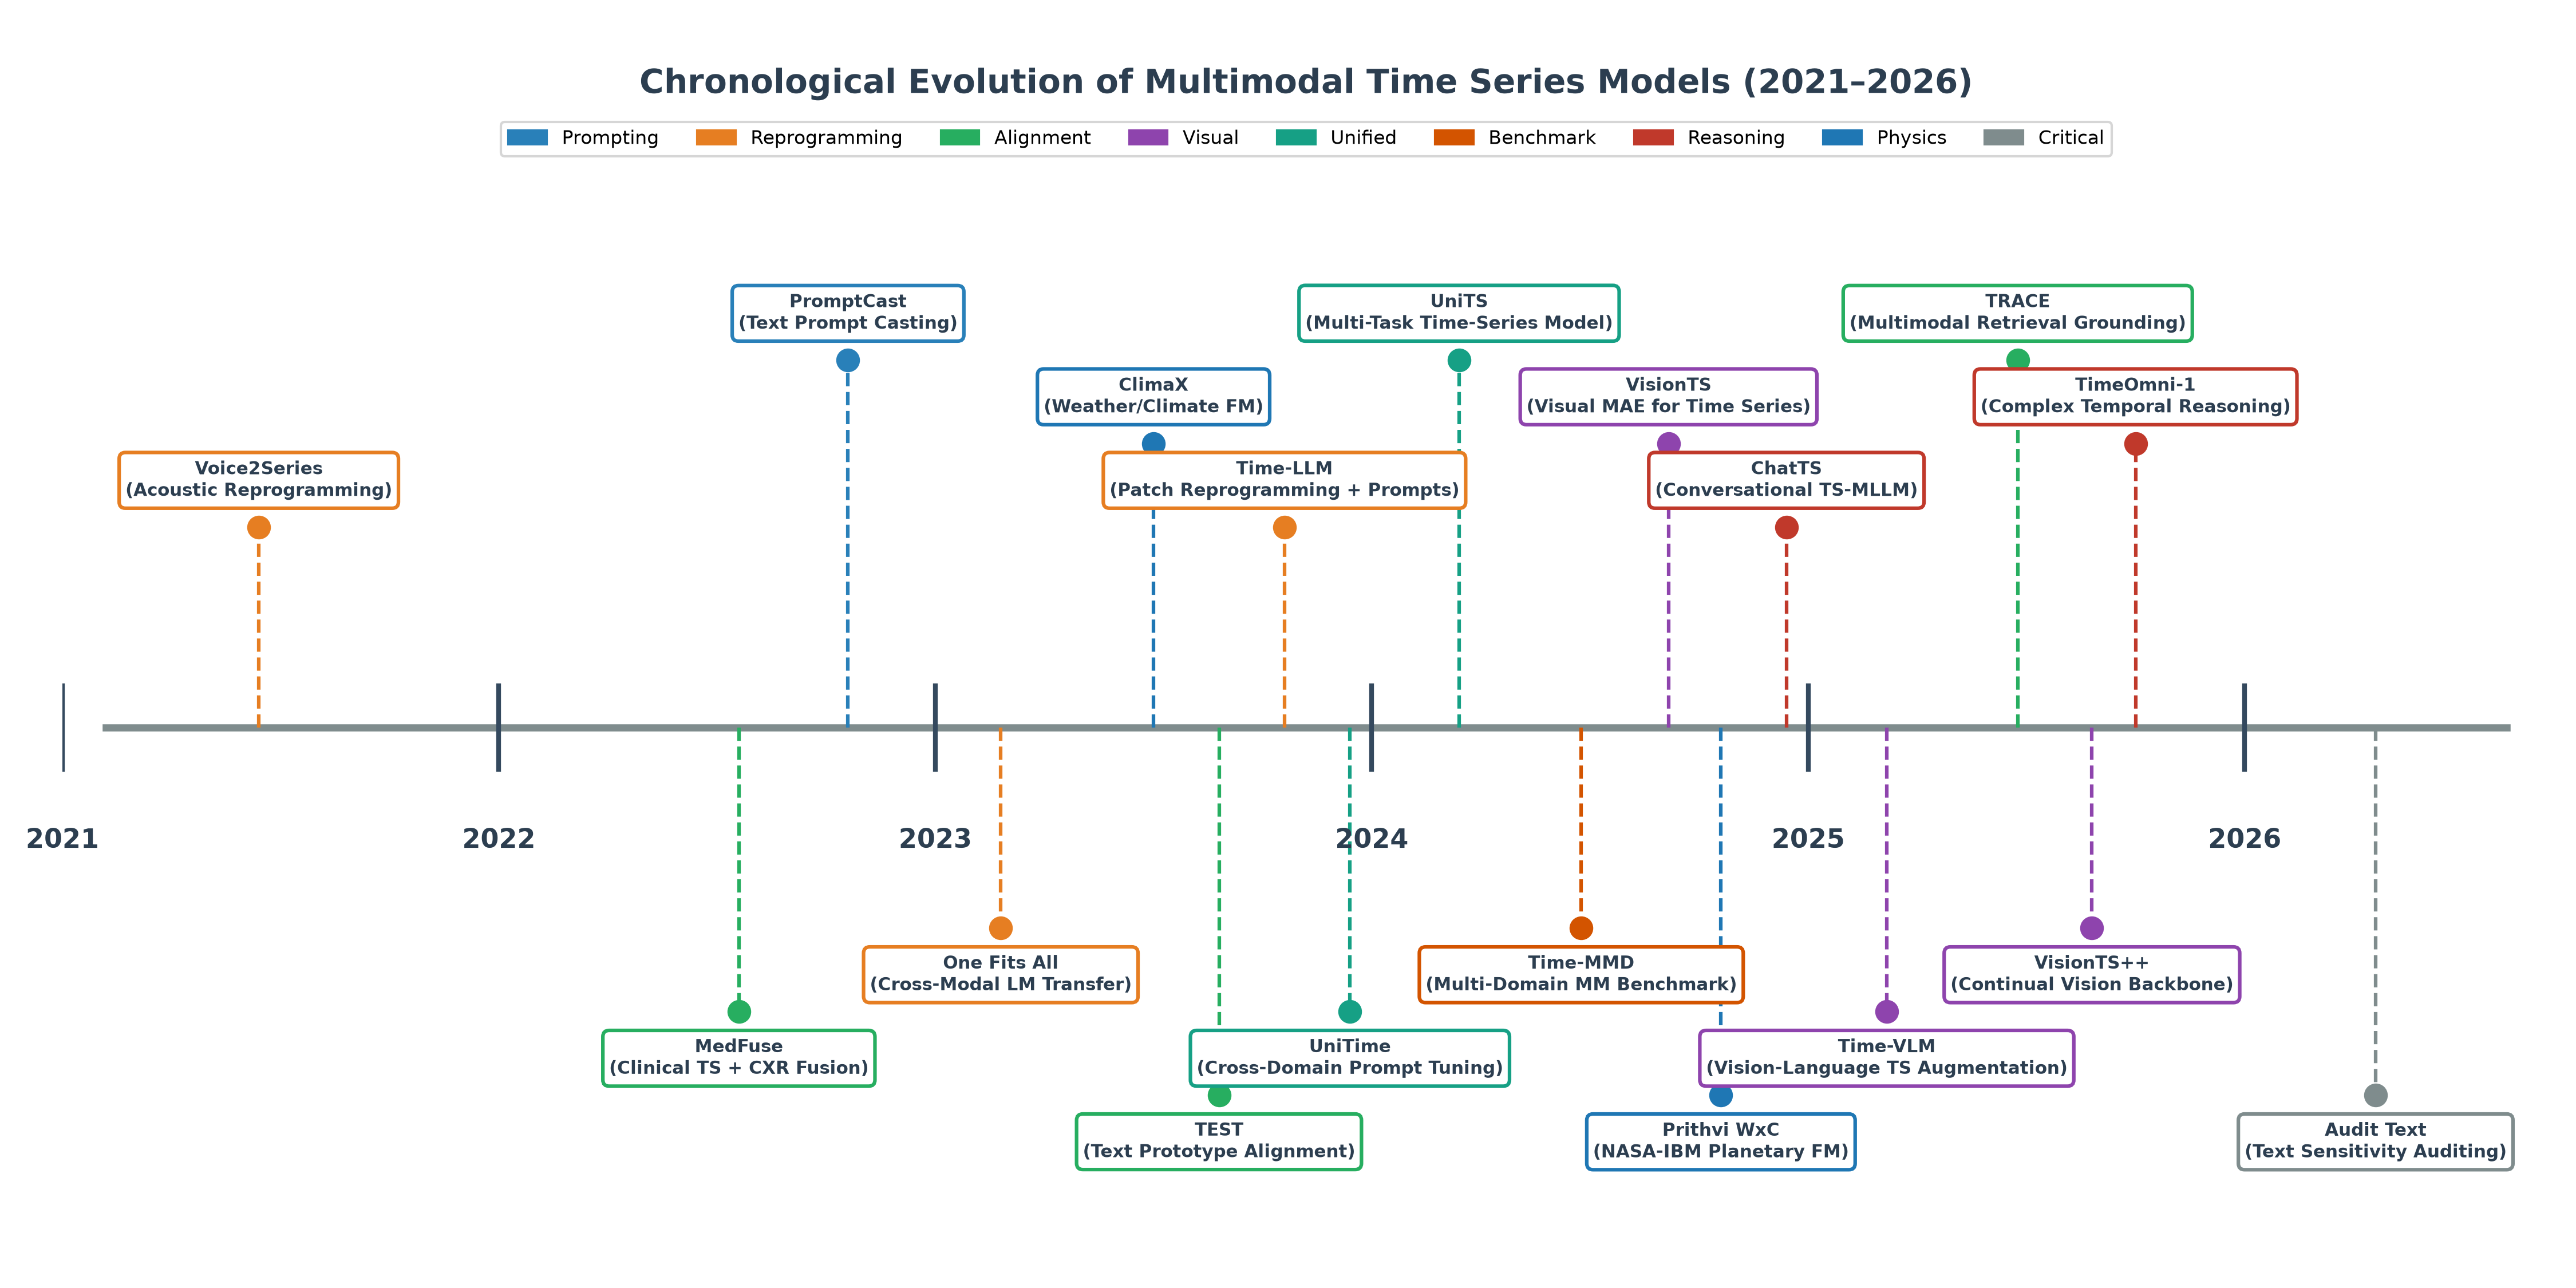
\includegraphics[width=0.98\textwidth]{figures/timeline_milestones.png}
\caption{Chronological milestones in multimodal time-series modeling from 2022 to 2026, illustrating the evolution from early text prompt casting (PromptCast) to cross-modal reprogramming (One Fits All, Time-LLM), visual transcoding (VisionTS), unified multimodal models (UniTS, Time-MMD), and neuro-symbolic reasoning frameworks (ChatTS, TimeOmni, Sonar-TS).}
\label{fig:timeline}
\end{figure*}

\subsection{Pillar 1: Modality Pairing}
The combinations of data modalities co-occurring with time series fundamentally dictate architectural constraints and inductive biases:
\begin{itemize}
    \item \textbf{Time Series + Text ($\text{TS} + \text{Text}$):} The most prominent paradigm. Text serves diverse functions: semantic descriptions (e.g., sensor metadata, sampling rates, geographical origins in Time-LLM~\cite{Jin2023TimeLLM} and TEMPO~\cite{Cao2023TEMPO}), continuous narrative reports (financial news, corporate filings, EHR medical notes in Time-MMD~\cite{Liu2024TimeMMD}), or natural language analytical queries~\cite{Zhao2024ChatTS,Xue2022PromptCast,Shen2025TimeMQA}.
    \item \textbf{Time Series + Vision ($\text{TS} + \text{Vision}$):} Exploits 2D visual representations—either by directly plotting numerical trajectories as line charts (VisionTS~\cite{Chen2024VisionTS}, VisionTS++~\cite{Chen2025VisionTSPlus}) or converting temporal signals into 2D spectrograms—to harness vision foundation models pre-trained on massive natural image corpora without manual task redesign.
    \item \textbf{Time Series + Audio / Acoustic Waveforms ($\text{TS} + \text{Audio}$):} Exemplified by Voice2Series~\cite{Yang2021Voice2Series} and SeisT~\cite{Zhang2024SeisT}. Continuous 1D acoustic and seismic waveforms share strong mathematical analogies with time series (e.g., frequency harmonics, non-stationary oscillatory wavelets), enabling cross-domain reprogramming from pre-trained speech/audio models.
    \item \textbf{Time Series + Spatio-Temporal Physical Grids ($\text{TS} + \text{Grid}$):} Foundational in Earth systems science (ClimaX~\cite{Nguyen2023ClimaX}, Prithvi WxC~\cite{Schmude2024PrithviWxC}, Aurora~\cite{Bodnar2024Aurora}). Here, multivariate temporal sequences are coupled with multi-level geospatial grids governed by atmospheric thermodynamics and fluid dynamics equations.
    \item \textbf{Time Series + Clinical Imaging ($\text{TS} + \text{Clinical}$):} MedFuse~\cite{Hayat2022MedFuse} couples irregularly sampled physiological ICU signals with paired chest X-rays, reconciling high-frequency temporal trajectories with static diagnostic scans.
    \item \textbf{Tri-Modal \& Omnimodal Systems ($\text{TS} + \text{Vision} + \text{Text}$):} Recent unified architectures, notably Time-VLM~\cite{Zhong2025TimeVLM} and TimeOmni-1~\cite{Tan2025TimeOmni1}, combine temporal sequences with synchronized visual views and textual context for holistic multi-sensory understanding.
\end{itemize}

\subsection{Pillar 2: Fusion Architecture}
How representations from disparate modalities are mathematically merged constitutes the core engineering challenge:
\begin{enumerate}
    \item \textbf{Cross-Modal Patch Reprogramming:} Keeps the backbone foundation model (e.g., LLaMA, GPT-2, acoustic nets) completely frozen. Patch-level linear or multi-head attention projection layers reprogram numerical time-series patches into the continuous embedding space of language or acoustic tokens~\cite{Yang2021Voice2Series,Jin2023TimeLLM,Zhou2023OneFitsAll,Chang2023LLM4TS,Liu2024CALF}.
    \item \textbf{Modality Transcoding \& Continual Vision Adaptation:} Transforms the temporal sequence into another modality prior to ingestion. VisionTS~\cite{Chen2024VisionTS} and VisionTS++~\cite{Chen2025VisionTSPlus} render normalized time series into pixel bitmaps, bypassing numerical tokenization entirely and processing the visual stream with ViT-based Masked Autoencoders.
    \item \textbf{Variable-Tokenized Physics Transformers:} Introduced by ClimaX~\cite{Nguyen2023ClimaX} and scaled by Prithvi WxC~\cite{Schmude2024PrithviWxC} and Aurora~\cite{Bodnar2024Aurora}. Heterogeneous physical variables are tokenized independently with variable-specific projection weights, enabling arbitrary subsets of variables, lead times, and spatial resolutions to be processed uniformly.
    \item \textbf{Decoupled Alignment \& Language Masking:} UniTime~\cite{Liu2024UniTime} and TimeCMA~\cite{Liu2024TimeCMA} employ language-masked cross-attention and cross-modal feature calibration, dynamically guiding temporal feature extraction without entangling raw time-series representations.
    \item \textbf{Unified Early Tokenization:} Maps heterogeneous modalities into a shared token dictionary. Models such as UniTS~\cite{Gao2024UniTS} and ChatTime~\cite{ChatTime2024} tokenize time-series patches, instruction prompts, and domain markers into unified token embeddings passed jointly into deep Transformer stacks.
    \item \textbf{Dual-Tower Metric Alignment:} Maintains separate, dedicated encoders for time-series and textual context, aligning them in a shared latent metric space using contrastive losses (e.g., TRACE~\cite{Chen2025TRACE} and TEST~\cite{Sun2023TEST}).
\end{enumerate}

\subsection{Pillar 3: Functional Role of the Complementary Modality}
Rather than treating all modalities symmetrically, the complementary modality plays specific functional roles:
\begin{itemize}
    \item \textbf{Auxiliary Context / Inductive Condition:} Text or metadata acts as conditioning information to resolve ambiguity in numerical time series, mitigating non-stationarity (e.g., Time-LLM, TEMPO, $\text{S}^2\text{IP-LLM}$~\cite{Pan2024S2IPLLM}, UniTime~\cite{Liu2024UniTime}).
    \item \textbf{Frozen Transfer Substrate:} The language or acoustic model acts as an overparameterized pattern-matching backbone whose self-attention mechanisms transfer directly to universal time-series forecasting (One Fits All~\cite{Zhou2023OneFitsAll}, Voice2Series~\cite{Yang2021Voice2Series}).
    \item \textbf{Physics / Geophysical Invariance Prior:} Multi-level atmospheric grids enforce physical continuity and conservation laws (ClimaX~\cite{Nguyen2023ClimaX}, Aurora~\cite{Bodnar2024Aurora}).
    \item \textbf{Conversational \& Reasoning Interface:} The non-TS modality serves as an interactive communication interface, enabling open-ended question answering, root-cause diagnostics, and counterfactual simulation (ChatTS~\cite{Zhao2024ChatTS}, TimeOmni-1~\cite{Tan2025TimeOmni1}, Time-MQA~\cite{Shen2025TimeMQA}).
    \item \textbf{Retrieval Anchor:} Text serves as a semantic query anchor for indexing, clustering, and retrieving dynamic time-series trajectories (TRACE~\cite{Chen2025TRACE}).
\end{itemize}

\subsection{Pillar 4: Downstream Tasks and Domains}
While unimodal models focus almost exclusively on point forecasting, multimodal frameworks support an expansive task portfolio:
\begin{itemize}
    \item \textbf{Multimodal Forecasting:} Point and probabilistic forecasting conditioned on both numerical history and external text/vision events.
    \item \textbf{Anomaly Detection \& Semantic Explanation:} Detecting out-of-distribution events and generating natural-language explanations of their causes.
    \item \textbf{Time-Series Question Answering (TS-QA):} Answering queries regarding periodic trends, maximum peaks, and correlated shifts (Time-MQA~\cite{Shen2025TimeMQA}, ChatTS~\cite{Zhao2024ChatTS}).
    \item \textbf{Earthquake Monitoring \& Phase Picking:} Detecting seismic P/S-wave arrivals and estimating hypocenters from multi-station seismic waveforms (SeisT~\cite{Zhang2024SeisT}).
    \item \textbf{Planetary Weather and Climate Forecasting:} Multi-horizon global prediction of surface temperature, geopotential height, and extreme weather phenomena (ClimaX, Prithvi WxC, Aurora).
    \item \textbf{Clinical Phenotyping \& Mortality Prediction:} Reconciling vitals time series and radiographs for ICU prognosis (MedFuse~\cite{Hayat2022MedFuse}).
    \item \textbf{Cross-Modal Retrieval:} Retrieving relevant time-series segments given natural language descriptions, and vice versa (TRACE~\cite{Chen2025TRACE}).
\end{itemize}
